\documentclass[./../SoftwareEngineering.tex]{subfiles}

\begin{document}
	\section{Thiết kế trong lĩnh vực lập trình}
	\textit{Thiết kế phần mềm }\index{thiết kế phần mềm} là một phần quan trọng của kỹ nghệ phần mềm và được áp dụng đối với tất cả các mô hình phát triển phần mềm. Các yêu cầu phần mềm ban đầu sẽ được phân tích và tiến hành mô hình hóa, thì thiết kế phần mềm chính là bước cuối cùng trong hoạt động mô hình hóa chuẩn bị cho giai đoạn xây dựng ( sinh mã nguồn và kiểm thử).
	

	
	\begin{figure}[!htb]
		\centering
		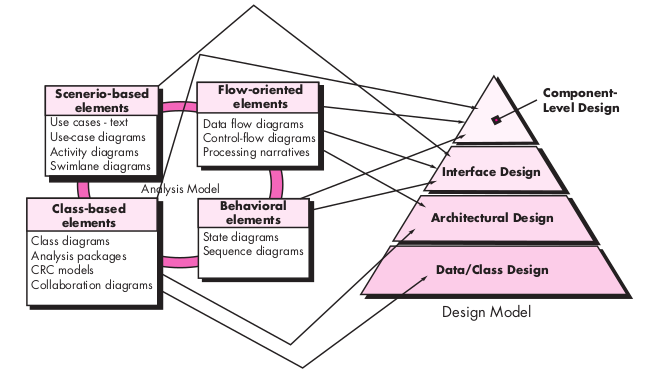
\includegraphics[width=\textwidth]{figure_8_1.png}
		\caption{Chuyển mô hình yêu cầu thành mô hình thiết kế}
		\label{fig:fig8_1}
	\end{figure}
	
	Luồng thông tin trong giai đoạn kĩ thuật này của tiến trình kỹ nghệ phần mềm được minh họa trong\autoref{fig:fig8_1}.Các yêu cầu phần mềm được biểu thị bởi mô hình luồng dữ liệu (flow-oriented elements), mô hình hành vi (behavioral elements), mô hình lớp (class-based elements), mô hình kịch bản (scenario-based). Bằng việc sử dụng một trong các phương pháp thiết kế, hoạt động thiết kế sẽ tạo ra:  thiết kế dữ liệu/lớp (data/class design), thiết kế kiến trúc(architectural design), thiết kế giao diện (interface design) và thiết kế thành phần (component-level design).
	
	

	\begin{description}
		\item[Thiết kế dữ liệu/lớp] chuyển mô hình lĩnh vực thông tin đã được tạo ra trong bước phân tích thành các cấu trúc dữ liệu sẽ cần cho việc thiết kế phần mềm. 
		\item[Thiết kế kiến trúc] xác định mối quan hệ giữa các thành phần cấu trúc chính của phần mềm.
		\item[Thiết kế giao diện] mô tả cách giao tiếp của một phần mềm với hệ thống và với người sử dụng. 
		\item[Thiết kế thành phần] các dịch vụ cung cấp cho các thành phần khác và các giao diện tương tác với chúng phải được thiết kế. 
	\end{description}
	
	
	Thiết kế, lập trình và kiểm thử chiếm đến 75 phần trăm chi phí kỹ nghệ phần mềm (trừ bảo trì). Chính tại các bước này mà chúng ta quyết định rằng sự thành công của việc cài đặt phần mềm sẽ bị ảnh hưởng hay là không, và điều quan trọng là làm dễ dàng cho việc bảo trì phần mềm. 
	
	
	
	Tầm quan trọng của thiết kế phần mềm có thể được phát biểu bằng một từ - \textit{chất lượng}. Thiết kế là nơi chất lượng được bồi dưỡng trong công nghệ phần mềm. Thiết kế cung cấp cho ta cách biểu diễn phần mềm có thể được xác nhận về chất lượng. Thiết kế là cách duy nhất để chúng ta có thể dịch chính xác các yêu cầu của khách hàng thành một sản phẩm hoặc hệ thống phần mềm hoàn chỉnh. Thiết kế phần mềm đóng vai trò là nền tảng cho tất cả các bước kỹ nghệ phần mềm và bảo trì phần mềm sau đó. Nếu không có thiết kế, ta có nguy cơ sẽ xây dựng nên một hệ thống không ổn định - một hệ thống sẽ thất bại khi có một thay đổi nhỏ; một hệ thống có thể khó mà thử nghiệm được; một hệ thống mà người ta không thể nào xác nhận được chất lượng cho đến khi thực hiện xong tiến trình kiểm thử, khi thời gian còn rất ngắn và đã tốn khá nhiều chi phí.
	

	
\end{document}